\chapter{First physics results from the binned analysis}
\label{results_diffuse}

\gls{anita} is a NASA long-duration balloon experiment for the detection of \gls{uhe} ($>10^{18}\,\mbox{eV}$) neutrinos. 
The third flight of the \gls{anita} experiment took place during Dec~19, 2014 to Jan~10, 2015. In this chapter, we present results of a search for a diffuse flux of \gls{uhe} neutrinos in data collected during this flight. These results have been made public now~\cite{diffuse}, however, in this chapter, we provide details that were not covered in the publication draft. 

\section{Short summary of published results}

Three independent blind searches for a diffuse flux of \gls{uhe} neutrinos and one dedicated search for \gls{eas} candidates were conducted. About 20 \gls{eas} candidates and one neutrino candidate were found. Their reconstructed locations overlaid on a map of the continent along with the \gls{anita}-3 flight path are shown in Figure~\ref{candidates}. The candidates are all impulsive, isolated events. The neutrino candidate is \gls{vpol} and the \gls{eas} candidates are \gls{hpol}. One of the \gls{eas} candidates is an unusual, upgoing event, referred to as the mystery event 2. This is further discussed in Chapter~\ref{wild}. 


%%%%%%%%%%%%%%%%%%%%%%%%%%%%%%%%%%%%%%%%%%%%%%%%%%%
\begin{figure}
\centering
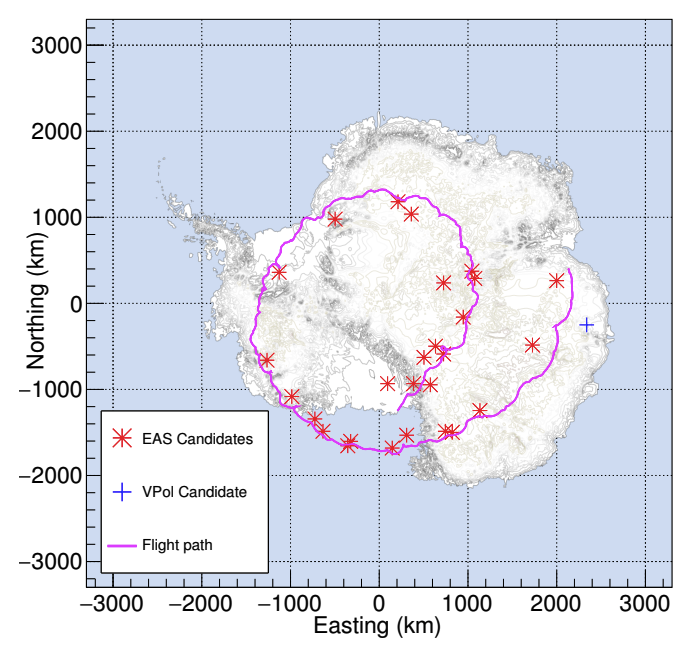
\includegraphics[width=0.6\textwidth]{figures/candidates.png}
\caption{Results from the ANITA-3 flight. Red stars denote EAS candidates. The blue plus denotes the neutrino candidate. These results are summarized in~\cite{diffuse}.}
\label{candidates} 
\par
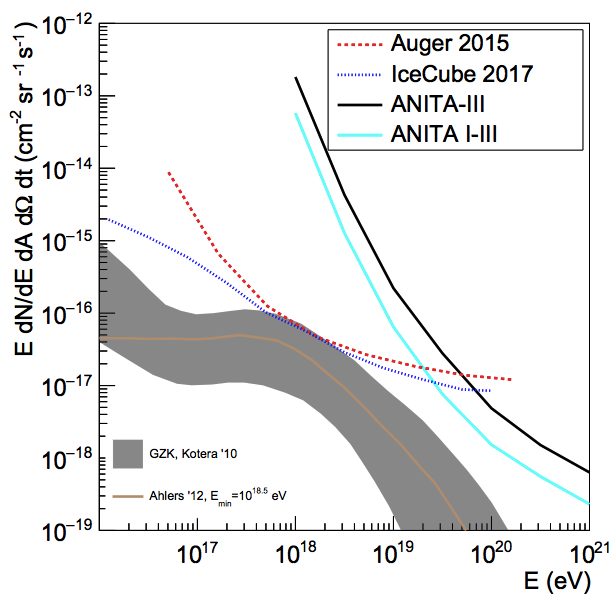
\includegraphics[width=0.64\textwidth]{figures/limit_diffuse.png}
\caption{New limit from a search for UHE neutrinos in data from the third flight of ANITA.}
\label{limit_diffuse}
\end{figure}
%%%%%%%%%%%%%%%%%%%%%%%%%%%%%%%%%%%%%%%%%%%%%%%%%%%


In the absence of a discovery, we present the new limit in Figure~\ref{limit_diffuse}. In this plot, there is flux in the vertical axis and energy in the horizontal axis. The neutrino background estimate quoted in the paper was: $0.7 ± ^{+0.5}_{-0.3}$, therefore, the neutrino candidate was consistent with background. However, an \textit{a posteriori} analysis found features of the neutrino candidate that will be used to improve future analyses. In Figure~\ref{limit_diffuse}, constraints from other experiments such as Auger and IceCube are also presented. Both the \gls{anita}-3 limit and the combined \gls{anita}-1 through -3 limit are shown. Note that there is a part of the range of energies in the horizontal axis where \gls{anita} is the only experiment with sensitivity. 

\section{What led to the first physics results in the binned analysis}

The binned analysis to search for a diffuse flux of \gls{uhe} neutrinos in the \gls{anita}-3 data was a team effort as evident from other theses ~\cite{samStaffordThesis,jacobGordonThesis}. 
Developments to find results from the 10\% data were presented in \cite{samStaffordThesis}.
Systematic uncertainties were added to the analysis in~\cite{jacobGordonThesis}.
The problem of excess background that was seen in previous attempts of the binned analysis as in~\cite{brianDaileyThesis} for \gls{anita}-2 and~\cite{samStaffordThesis} for \gls{anita}-3 was also largely corrected by incorporating conservative cuts such as the satellite stripe cut which is described in Chapter~\ref{analysis}. A critical problem remained, which was the loss of sensitivity. 

\subsection{Improving sensitivity in the binned analysis}

Increasing the sensitivity of the binned analysis played a critical role in publishing the first physics results from this analysis. Here, sensitivity means keeping ice where we are sensitive to neutrinos. Before I started working on improving the sensitivity of the analysis, the sensitivity in the \gls{hpol} channel of the analysis was 27\% and the sensitivity in the \gls{vpol} channel of the analysis was 44\%. This was partly due to removing many bins from the analysis. Twelve bins were being kept in the \gls{hpol} channel and 22 bins were being kept in the \gls{vpol} channel of the analysis. It was important to improve these numbers. 

\begin{figure}
\centering
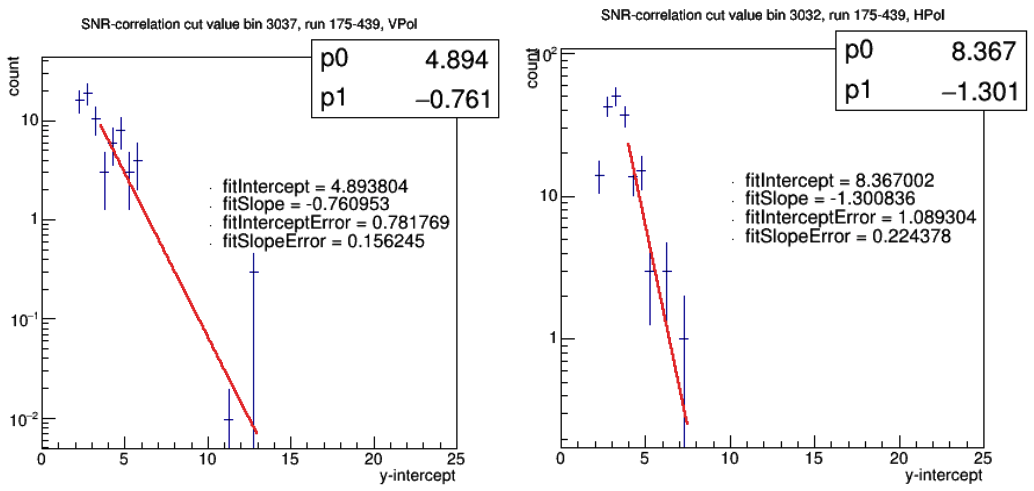
\includegraphics[width=1.0\textwidth]{figures/expo_fixed.png}
\caption{Exponential fit for LD cut was updated. Now, the fit has to have at least 5 histogram bins
with data and with at least 5 total events.}
\label{expo_fixed}
\end{figure}

\subsubsection{Updating the exponential fit requirements}

Improving the logic for deciding which bins fulfill the requirements needed before of having their data be fit to an exponential helped to increase the sensitivity of the binned analysis. As has been explained before, at a later stage of the binned analysis, the y-intercept of the LD cut of data in each bin is fit to an exponential as part of the optimization process of the LD cut and only bins that satisfy certain rules can be fit to an exponential. 

I updated the rules to allow a Healpix bin to be kept if the exponential fit to its data has at least five histogram bins and if the distribution has at least five total events. Previously, bins where consecutive histogram bins in the fit did not have data were rejected. Also, bins where the values of the histogram bin content were not in descending order were rejected. Figure~\ref{expo_fixed} shows two such bins that would have failed the previous rules, but that are now acceptable and thus, would be kept in the analysis. 

\subsubsection{Keeping high background bins}

Keeping bins that were being rejected previously for having higher background also helped to improve the sensitivity of the binned analysis. Bins with background greater than 1 were not being kept in the analysis before. I forced the background of these bins down to 0.1 by increasing the LD cut in these bins by hand instead of using their optimized LD cut. Figure~\ref{high_bg_kept} shows one such bin that would have been rejected before due to higher background, but was kept in the analysis now. 

This allowed for a very strong signal, if present in such a bin, to be found by the binned analysis as it would have to pass the stricter LD cut. In many cases, however, the LD cut had to be made only a little bit stricter, for example, from 10 to 11, as the background in that bin was just over 1. Keeping such bins only made sense and helped the analysis overall. 

\begin{figure}
\centering
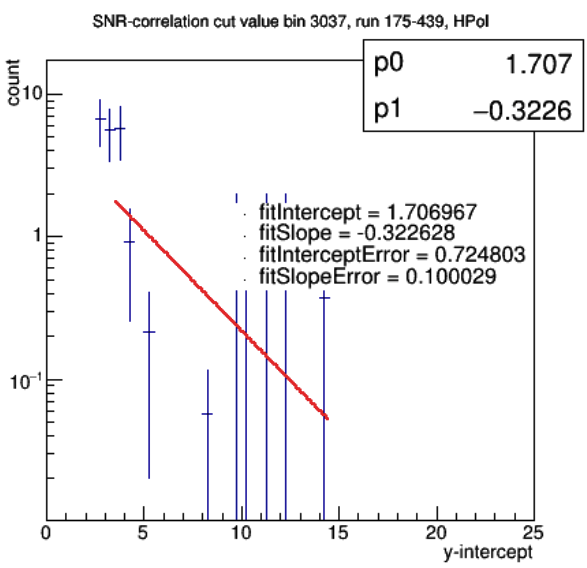
\includegraphics[width=0.65\textwidth]{figures/high_bg_kept.png}
\caption{Bins with high background ($>1$) now get
optimized cut tuned to allow expected
background of 0.1.}
\label{high_bg_kept}
\end{figure}

\subsubsection{Summary}

To summarize, I updated the requirements for which bins satisfied the rules for getting fitted to an exponential, and started to keep bins with higher background by forcing their LD cuts to be stricter. These helped to increase the number of bins in the analysis. Now I could keep 29 bins in the \gls{hpol} channel and 37 bins in the \gls{vpol} channel. Consequently, this improved the sensitivity of the analysis and now the numbers were 75\% in the \gls{hpol} channel and 63\% in the \gls{vpol} channel. These are summarized in Table~\ref{improvement}. \\

\begin{table}
\centering
\begin{tabular}{ |c|c|c|c|c| } 
\hline
  & Bins kept in H  & Bins kept in V  & Sensitivity in H & Sensitivity in V \\ 
\hline
 Before & 12 & 22 & 27\% & 44\% \\ 
 After & 29 & 37 & 75\% & 63\% \\ 
\hline
\end{tabular}
\caption{Before and after summary showing improvement of the binned analysis.}
\label{improvement}
\end{table}


\section{Background estimate}

The background was estimated for each bin in the \gls{vpol} box using a simple extrapolation of the exponential fit for that bin. As described in Chapter~\ref{analysis}, the distribution of y-intercepts associated with events in each bin was fit to an exponential distribution. An estimate of the background was calculated for each bin following the relation in Equation~\ref{background}. 


\begin{equation*}
Background = \frac{-0.9}{sampleFrac * fitSlope * w}
\exp(fitSlope * optCutVal + fitIntercept) \\
\label{background}
\end{equation*}


The number of background events expected to pass final cuts in each bin used in the \gls{vpol} analysis is shown in Figure~\ref{bg_est}. This plot shows the estimated background in each bin with a solid black bar. The number of simulated neutrinos passing final cuts in the same bins is shown with shaded orange bars. The number of simulated neutrinos passing in a bin is a measure of the sensitivity of that bin to neutrinos. Here, the number of simulated neutrinos is in arbitrary units. 

It can be seen from Figure~\ref{bg_est} that a variety of bins were kept in the \gls{anita}-3 binned analysis. Some bins had a larger number of expected background events than others. Some bins had greater sensitivity to neutrinos than others. This is the key difference between the binned analysis and other complementary analyses: parts of the continent with more noise can be retained in the binned analysis using a stricter LD cut than parts of the continent with less noise, with the goal of keeping as much of the continent as possible where we are sensitive to neutrinos. 

The LD cut used in each bin kept in the \gls{vpol} analysis is shown in Figure~\ref{ldcut_pop} as a function of the number of events in that bin before final cuts. Final cuts include the LD cut, bin cut, and event bin-weight cut. It can be seen that the distribution of LD cuts is mostly flat with a few being larger than others. 


\begin{figure}
\centering
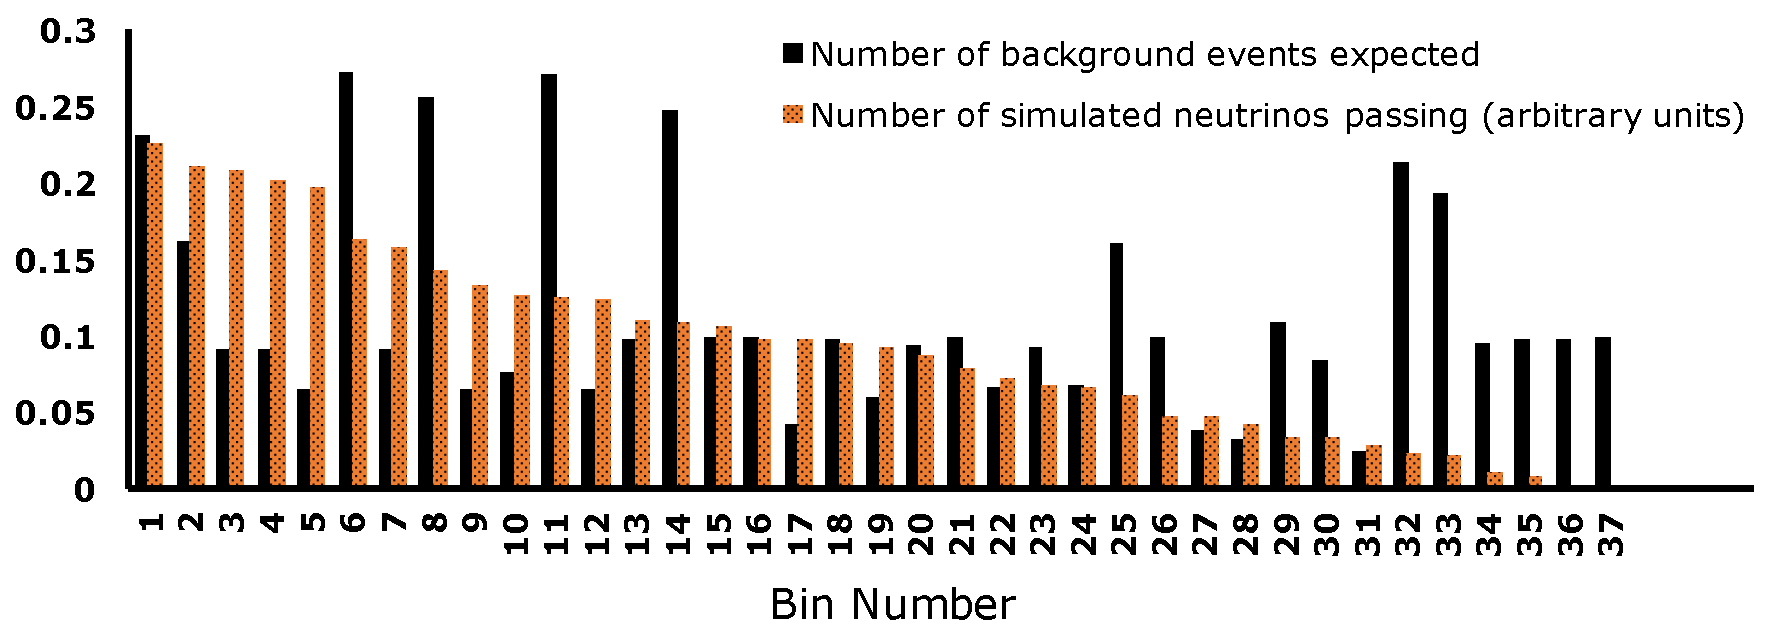
\includegraphics[width=1.0\textwidth]{figures/background_simpassing_vpol_bins.pdf}
\caption{Distribution of background estimates (solid black bars) and number of simulated neutrinos passing (shaded orange bars) final cuts in each bin used in the VPol box. }
\label{bg_est}
\end{figure}


\begin{figure}
\centering
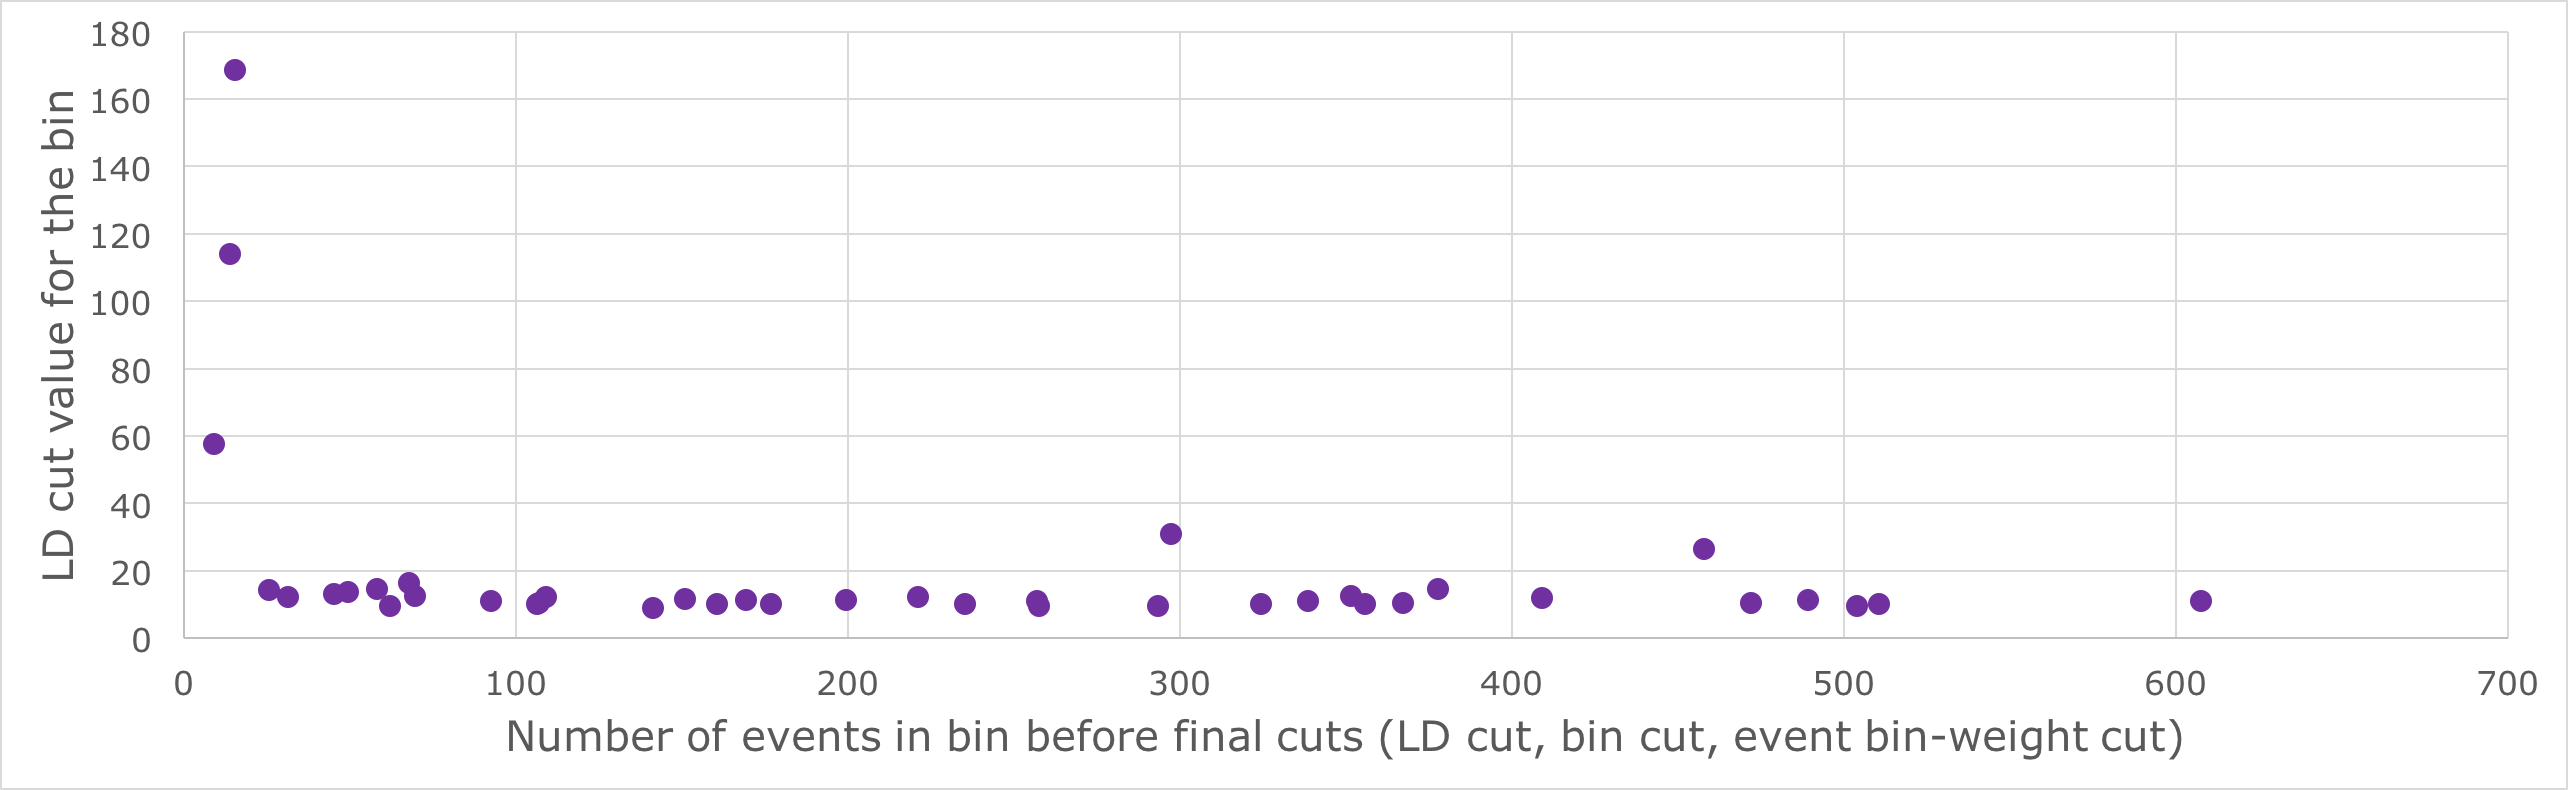
\includegraphics[width=1.0\textwidth]{figures/LDcutVsEventPopulationBeforeFinalCuts.png}
\caption{Distribution of LD cuts as a function of number of events in the bin before final cuts. }
\label{ldcut_pop}
\end{figure}


\section{Box opening results in the binned analysis}

The binned analysis was one of the three independent blind analyses performed on the \gls{anita}-3 data to search for a diffuse flux of \gls{uhe} neutrinos~\cite{diffuse}. Analysis cuts were determined using only 10\% of the data. To find candidates, the data was unblinded in this analysis in three stages: \gls{hpol} box opening, \gls{vpol} sideband box opening, and \gls{vpol} box opening. 

The \gls{hpol} box consists of events in the 90\% data that are horizontally polarized. In general, neutrinos are not expected in the \gls{hpol} box. \gls{eas} candidates, however, are. The binned analysis did not optimize its search to find \gls{eas} candidates. We used 29 bins in the \gls{hpol} box. 

The sideband channel consists of events in the 90\% data that reconstruct to bins that account for less than 1\% of the cumulative sensitivity and are usually ones lacking ice depth. There was no \gls{hpol} sideband channel is this search, that is, no events in the 90\% \gls{hpol} channel that reconstructed to zero sensitivity bins.  There were four bins in the sideband \gls{vpol} channel. 

The \gls{vpol} box consists of events in the 90\% data that are vertically polarized. This is the most important box in this search. The \gls{vpol} box is where neutrinos would be expected. We used 37 bins in the \gls{vpol} box. 

Before opening the \gls{hpol} and \gls{vpol} boxes, we decided to remove certain types of events if they were found: payload blasts or events that obviously require a quality cut, and clustering events. 
It is challenging to design cuts that remove all payload blasts.
These types of events were known to pass quality and analysis cuts before. So, we decided that if we found such events in the boxes, we would remove them by hand. This simply means that we would look at the waveforms of the events and if they had the distinct features of payload blasts or other low-quality events, they would be removed. We also reserved the right to remove any groups of events in the boxes that appeared to be part of a cluster. A cluster is a group of events that are near each other (within 40 km). Such events are typically associated with anthropogenic noise and deemed worthy of removal. 


\begin{figure}
\centering
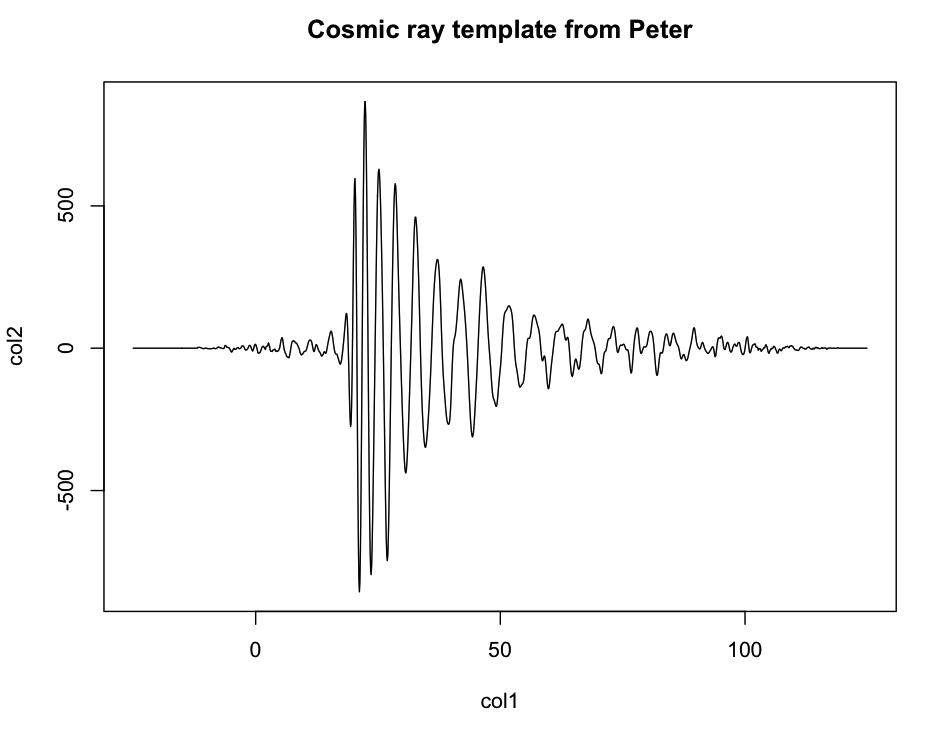
\includegraphics[width=1.0\textwidth]{figures/CRtemplate.png}
\caption{Cosmic ray template used in~\cite{me2}. P. Gorham provided the numbers to make this figure.}
\label{cr_template}
\end{figure}


\subsection{Cosmic ray candidates and cRay scores}

Although primarily commissioned as a neutrino detector, \gls{anita} is sensitive to radio signatures of \gls{uhecrs} and have made observations of \gls{cr} events in the \gls{hpol} channel of all analyses. Indeed the \gls{hpol} channel of the signal box is mainly expected to yield \gls{cr} candidates, not neutrinos. The exception to this general expectation comes in the form of the mystery events that are discussed in Chapter~\ref{wild}. 

The binned analysis to search for a diffuse flux of \gls{uhe} neutrinos in the \gls{anita}-3 data was focused on finding the best limit on a diffuse neutrino flux, and not on finding \gls{cr} candidates. The \gls{hpol} channel of the binned analysis was treated the same as the \gls{vpol} channel in spite of the difference in the type of candidate expected in each. 

A complementary analysis described in~\cite{me2} was dedicated to a search for \gls{cr} candidates. In this analysis, a template matching technique was implemented to search for \gls{cr} candidates. The \gls{cr} template utilized in the analysis is shown in Figure~\ref{cr_template}. According to this analysis, this is what a \gls{cr} candidate should look like. By comparing processed waveforms of events recorded in the flight to this template, an evaluation was made on how \gls{cr}-like they were. This evaluation was presented as a number, known as the cRay score, for each event. Events with cRay scores above 0.55 were chosen as \gls{cr} candidates. Note that to be a \gls{cr} candidate the event also had to pass all other cuts in the analysis, most importantly, the clustering cut. 

In the binned analysis, events passing final cuts in the \gls{hpol} channel were put through the procedure of comparison with the \gls{cr} template and a cRay score was determined for each one. These results are summarized in Table~\ref{isolated_table} and discussed in Section~\ref{hpol_box_open}.  


\subsection{HPol box opening results}
\label{hpol_box_open}

On opening the \gls{hpol} box consisting of 29 bins, three types of events were found: isolated events, events that required a clustering cut, and payload blast events. 
There were seven isolated events, seven payload blast events, and 27 clustering events. These events came from both bins where the LD cut was optimized, referred to as ``normal bins" and bins where the LD cut, after optimization, was increased due to high  background ($>1$) in the bin to reduce the latter to 0.1, referred to as ``high background bins".

Of the seven isolated \gls{hpol} candidates, three were accepted by the collaboration as \gls{cr} candidates. Two of these were also found in complementary analyses, with one coming from a normal bin and the other from a high background bin in this analysis. 

Two new \gls{cr} candidates were found in the binned analysis. Both events 48837708 and 56038445 were rejected by other searches due to their clustering cut, with 48837708 being closer to the chosen clustering threshold than 56038445. This led to 48837708 being deemed acceptable as a \gls{cr} candidate by the collaboration while 56038445 was not. Event 48837708 was listed as a \gls{cr} in the publication~\cite{diffuse}, while 56038445 was not. Note, however, that both have cRay scores above 0.55. 

Both events 48837708 and 56038445 were found in high background bins in the binned analysis. This confirms that it was a good idea to keep the high background bins in the binned analysis. 
We summarize results from the \gls{hpol} box opening, starting with the isolated events in Table~\ref{isolated_table}. 

%%%%%%%%%%%%%%%%%%%%%%%%%%%%%%%%%%%%%%%%%%%%%%%%%%
%%%%%%%%%%%%%%%%%%%%% isolated hpol %%%%%%%%%%%%%%
\begin{table}
\centering
\begin{tabular}{ |c|c|c|c|c|c|c|c|c| } 
 \hline
Event & Pol & Run & Bin & Weight & Lat & Lon & cRay[4] & Notes \\
\hline
48837708 & H & 311 & 3057 & 1.0 & -79.1 & -72.3 & 0.8 &{\color{red} New CR candidate} \\
56038445 & H & 334 & 3042 & 0.6 & -79.9 & -123.1 & 0.7 & New CR candidate \\
58592863 & H & 343 & 3025 & 1.0 & -76.9 & -118.5 & 0.8 & {\color{blue} CR candidate} \\
33484995 & H & 250 & 3048 & 1.0 & -80.3 & 19.4 & 0.7 & {\color{blue} CR candidate} \\	
59130831 & H & 346 & 3042 & 1.0 & -77.2 & -128.5 & 0.4 & cRay score $<0.6$ \\	
15478875 & H & 175 & 3052 & 1.0 & -82.7 & 124.1 & 0.5 &	cRay score $<0.6$\\
30306654 & H & 241 & 3033 & 1.0 & -77.7 & 26.2 & 0.3 & cRay score $<0.6$	 \\
\hline
\end{tabular}
\caption{Isolated events found from opening the HPol box. The top event is not found in other analyses and is found in the binned analysis in a bin that was kept after increasing the LD cut. This event was published as a CR candidate. The events in blue font are CR candidates in other analyses as well. The fourth CR candidate was not deemed CR enough by other analysts and did not make the CR list in the publication. Three of the isolated events had CRay scores below $0.6$, the chosen cutoff.}
\label{isolated_table}
\end{table}
%%%%%%%%%%%%%%%%%%%%%%%%%%%%%%%%%%%%%%%%%%%%%%%%%%
%%%%%%%%%%%%%%%%%%%%% isolated hpol %%%%%%%%%%%%%%

%%%%%%%%%%%%%%%%%%%%%%%%%%%%%%%%%%%%%%%%%%%%%%%%%%%
%%%%%%%% HPOL events that had to be removed %%%%%%%%%
%%%%%%%%%%%%%%%%%% normal bins%%%%%%%%%%%%%%%%%%%%%%%


\begin{figure}
\centering
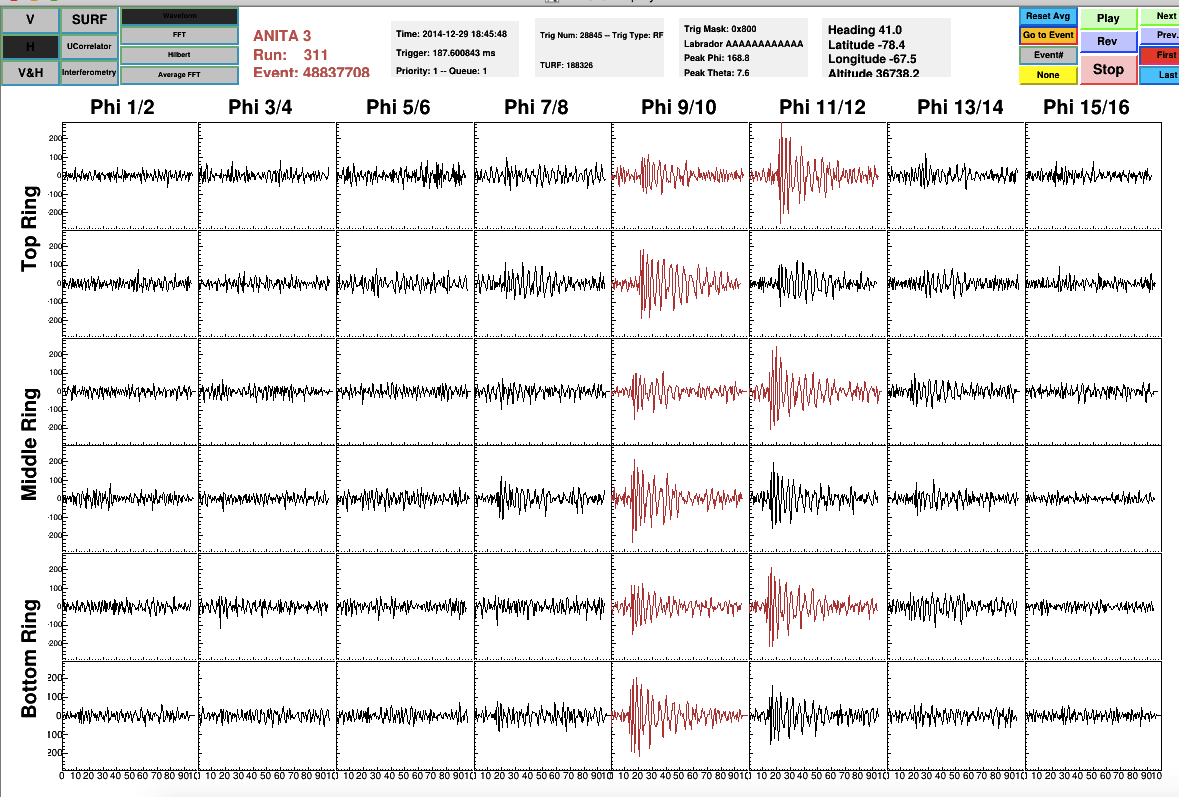
\includegraphics[width=0.9\textwidth]{figures/48837708.png}
\caption{The new cosmic ray candidate that I found that was published as such~\cite{diffuse}.}
\label{new_cr}
\end{figure}


\begin{figure}
\centering
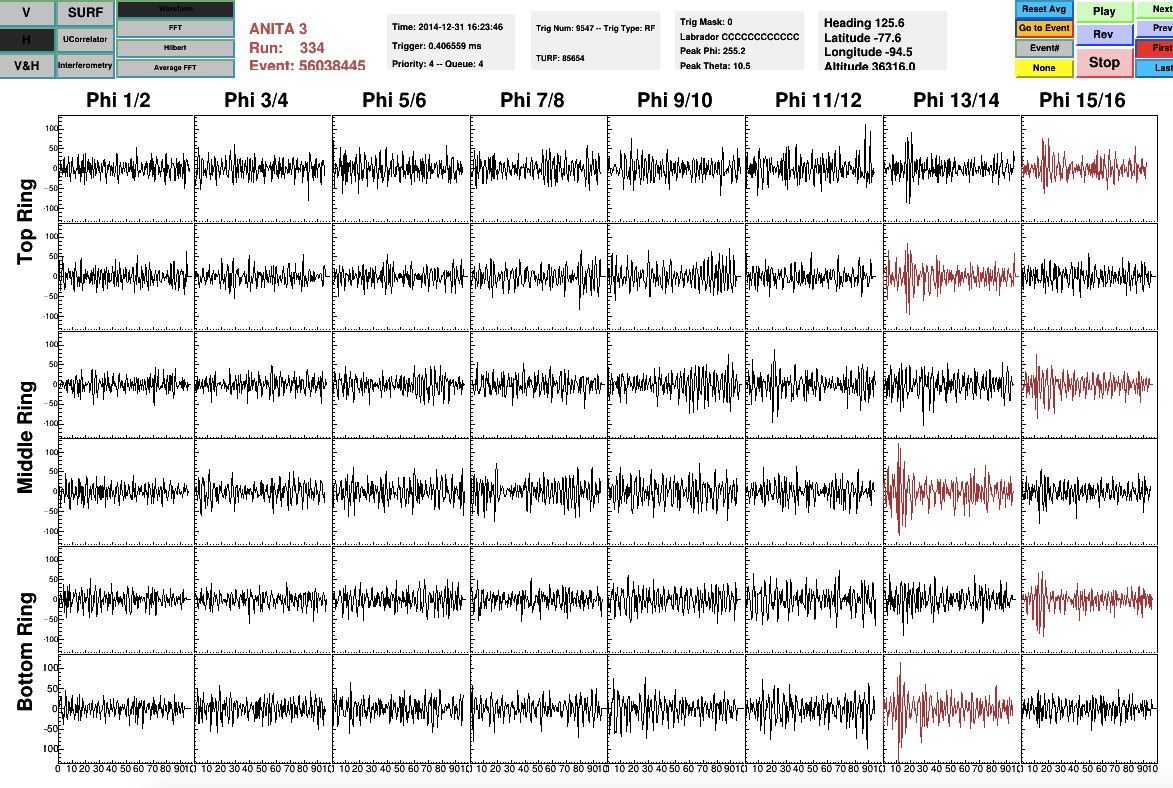
\includegraphics[width=0.9\textwidth]{figures/56038445.png}
\caption{Cosmic ray candidate that I found that did not make the list of CR candidates in publication~\cite{diffuse}.}
\label{cr_but_reject}
\end{figure}


Events that needed a clustering or quality (blast) cut were found in both the normal and the high background bins. 
Events that needed a clustering or quality (blast) cut after opening the \gls{hpol} box of normal bins are presented in Table~\ref{normal_hpol_bins}. 
It can be seen that five blasts and 11 clustering events were found in the normal bins. All of the clustering events in this group were part of a tight cluster and reconstructed to a single bin, Bin 3046. 
Events that needed a clustering or quality (blast) cut after opening the \gls{hpol} box of high background bins are presented in Table~\ref{high_bg_hpol_bins}. Two blasts and 16 clustering events were found in the high background bins. Six of the clustering events reconstructed to Bin 3057 and three to Bin 3024. Doublets were found in Bins 3018 and 2997. The clustering event from Bin 3019 clustered with the event 77973578 that passed in the 10\% dataset.

We present a table of \gls{eas} candidates found by complementary analyses and note the reason why we cut an event if it was removed in the binned analysis in Table~\ref{othersCRs}. Of the 23 total \gls{eas} candidates found in other analyses, two events were also found by the binned analysis. Five events were cut by the satellite stripe cut and three by the elevation angle cut. Five were removed due to the LD cut and six due to the bin cut. One was removed due to the reconstruction to continent cut and lastly, one by the triggering phi-sector direction cut. The LD cut and bin cut are unique to the methods of the binned analysis, therefore, it 
is not too surprising that \gls{eas} candidates were found by other analyses that were removed in the binned analysis due to these cuts. A brief discussion on the cuts that removed the other \gls{eas} candidates is presented in Section~\ref{conservative}. 



\begin{table}
\centering
\begin{tabular}{ |c|c|c|c|c|c|c|c| } 
\hline

Event & Pol & Run & Bin & Weight & Lat & Lon & Notes \\
\hline
15406158 & H & 175 & 3052 & 1.0 & -83.0 & 126.4 & {\color{red} Blast} \\
20646656 & H & 202 & 3035 & 1.0 & -80.4 & 83.4 & {\color{red} Blast} \\
23937896 & H & 216 & 3050 & 1.0 & -80.5 & 59.7 & {\color{red} Blast} \\
28876488 & H & 236 & 3049 & 1.0 & -79.2 & 37.6 & {\color{red} Blast} \\
82011215 & H & 429 & 2994 & 1.0 & -71.5 & 97.8 & {\color{red} Blast} \\
40579667 & H & 280 & 3046 & 1.0 & -77.8 & -34.3 & Clusters \\
40993619 & H & 281 & 3046 & 1.0 & -77.8 & -34.3 & Clusters \\
41049372 & H & 281 & 3046 & 1.0 & -77.9 & -34.3 & Clusters \\
41064920 & H & 281 & 3046 & 1.0 & -77.9 & -34.2 & Clusters \\
41073934 & H & 281 & 3046 & 1.0 & -77.8 & -34.4 & Clusters \\
41103084 & H & 281 & 3046 & 1.0 & -77.8 & -34.3 & Clusters \\
44543143 & H & 296 & 3046 & 1.0 & -77.8 & -34.3 & Clusters \\ 
44600768 & H & 296 & 3046 & 1.0 & -77.8 & -34.4 & Clusters \\
44677846 & H & 296 & 3046 & 1.0 & -77.9 & -34.6 & Clusters \\
44678128 & H & 296 & 3046 & 1.0 & -77.9 & -34.6 & Clusters \\ 
44678408 & H & 296 & 3046 & 1.0 & -77.8 & -34.5 & Clusters \\

\hline
\end{tabular}
\caption{Events that needed a clustering or quality (blast) cut in the bins kept in the HPol box that used a normal LD cut.}
\label{normal_hpol_bins}
\end{table}
%%%%%%%%%%%%%%%%%% normal bins%%%%%%%%%%%%%%%%%%%%%%%
%%%%%%%%%%%%%%%%%% high bg bins %%%%%%%%%%%%%%%%%%%%%%%

\begin{table}
\centering
\begin{tabular}{ |c|c|c|c|c|c|c|c| } 
\hline

Event & Pol & Run & Bin & Weight & Lat & Lon & Notes \\
\hline
74047179 & H & 399 & 2998 & 1.0 & -74.2 & 153.8 & {\color{red} Blast}\\
80333037 & H & 422 & 2995 & 1.0 & -71.8 & 107.9 & {\color{red} Blast}\\
19567583 & H & 196 & 3018 & 1.0 & -77.5 & 110.0 & Clusters\\ 
19567584 & H & 196 & 3018 & 1.0 & -77.7 & 109.4 & Clusters\\
78361533 & H & 415 & 3019 & 1.0 & -75.8 & 125.2 & Clusters w/ 10\%\\
76096974 & H & 407 & 2997 & 1.0 & -73.5 & 136.2 & Clusters\\ 
77072568 & H & 410 & 2997 & 1.0 & -73.8 & 136.3 & Clusters\\ 
63842646 & H & 362 & 3024 & 1.0 & -76.3 & -144.4 & Clusters\\ 
64166505 & H & 364 & 3024 & 1.0 & -76.3 & -144.4 & Clusters\\ 
64216077 & H & 364 & 3024 & 1.0 & -76.3 & -144.4 & Clusters\\
77136488 & H & 410 & 3037 & 1.0 & -75.7 & 122.0 & Clusters\\
77320292 & H & 411 & 3037 & 0.6 & -75.6 & 122.7 & Clusters\\
55584513 & H & 332 & 3057 & 0.7 & -79.9 & -82.2 & Clusters\\
55616654 & H & 332 & 3057 & 0.5 & -79.9 & -81.9 & Clusters\\ 
55827553 & H & 333 & 3057 & 0.8 & -79.9 & -81.6 & Clusters\\
56128670 & H & 334 & 3057 & 0.9 & -79.9 & -81.4 & Clusters\\
56141471 & H & 334 & 3057 & 0.5 & -79.9 & -81.7 & Clusters\\
56142587 & H & 334 & 3057 & 0.6 & -79.8 & -81.8 & Clusters\\
\hline
\end{tabular}
\caption{Events that needed a clustering or quality (blast) cut in the bins kept in the HPol box where the LD cut had to be increased manually to reduce the background to 0.1.}
\label{high_bg_hpol_bins}
\end{table}
%%%%%%%%%%%%%%%%%% high bg bins %%%%%%%%%%%%%%%%%%%%%%%
%%%%%%%%%%%%%%%%%%%%%%%%%%%%%%%%%%%%%%%%%%%%%%%%%%%
%%%%%%%% HPOL events that had to be removed %%%%%%%%%


%%%%%%%%%%%%%%%%%%%%%%%%%%%%%%%%%%%%%%%%%%%%%%%%%%%%
%%%%%%%%%%%%%% other's eas candidates %%%%%%%%%%%%%%
\begin{table}
\centering
\begin{tabular}{ |c|c|c| } 
 \hline
	Run number & Event number & Notes \\
    \hline
    343	&  58592863  &  {\color{blue} Passed in our analysis}\\
    250	 & 33484995  &  {\color{blue} Passed in our analysis}\\
    215	 & 23695286  &  Satellite stripe cut\\
    248	 & 32907848  &  Satellite stripe cut\\
	282	 & 41475569  &  Satellite stripe cut\\
    389	&  71766273  &  Satellite stripe cut\\
	401	&  74592579  &  Satellite stripe cut\\
	176	 & 15717147  &  Elevation angle cut\\
    371	&  66313844  &  Elevation angle cut\\
	377	&  68298837  &  Elevation angle cut\\
    210	&  22345215  &  Triggering phi-sector direction cut\\
    230	 & 27142546  &  Reconstruct to continent cut\\
	185	 & 16952229  &  LD cut\\
	195	 & 19459851  &  LD cut\\
    424	&  80840274  &  LD cut\\
    357	&  62273732  &  LD cut\\
	404	&  75277769  &  LD cut\\
    367	&  65187079  &  Bin cut\\
	388	&  71171108  &  Bin cut\\
	284	&  41529195  &  Bin cut\\
	435	&  83877990  &  Bin cut\\
	383	&  70013898  &  Bin cut\\
	397	&  73726742  &  Bin cut\\
\hline
\end{tabular}
\caption{EAS candidates that passed in complementary, independent analyses and notes mentioning whether they were found in the ANITA-3 binned analysis and the cut that removed them if they were not.}
\label{othersCRs}
\end{table}
%%%%%%%%%%%%%%%%%%%%%%%%%%%%%%%%%%%%%%%%%%%%%%%%%%%%
%%%%%%%%%%%%%% other's eas candidates %%%%%%%%%%%%%%


\subsection{VPol sideband results}

The \gls{vpol} sideband consisted of four bins: Bins 2975, 2978, 2900, and 3001. Nothing was found to pass in Bin 2900. One event, a payload blast event (64175392), was found in Bin 3001. Bins 2975 and 2978 had events that needed a clustering cut and are summarized in Table~\ref{sideband}.

\begin{table}
\centering
\begin{tabular}{ |c|c|c|c|c|c|c|c| } 
\hline
Event & Pol & Run & Bin & Weight & Lat & Lon & Notes \\
\hline
59664991 & V & 348 & 2978 & 1.0 & -77.0 & -120.3 & Clusters\\
59827186 & V & 348 & 2978 & 0.9 & -76.1 & -124.4 & Clusters\\
63140350 & V & 360 & 2978 & 0.6 & -76.8 & -122.1 & Clusters\\
66702609 & V & 372 & 2975 & 1.0 & -74.2 & -163.6 & Clusters\\
66703250 & V & 372 & 2975 & 1.0 & -74.2 & -163.5 & Clusters\\
66993765 & V & 372 & 2975 & 0.5 & -73.9 & -165.7 & Clusters\\
66998800 & V & 372 & 2975 & 1.0 & -73.9 & -165.7 & Clusters\\
\hline
\end{tabular}
\caption{Events that needed a clustering cut in the bins kept in the VPol sideband.}
\label{sideband}
\end{table}


\subsection{VPol box opening results}

On opening the \gls{vpol} box consisting of 37 bins, three types of events were found: isolated events, events that required a clustering cut, and events that required a quality cut. Twenty-eight total events were found to require a quality cut, of which there were 26 blasts, one reverse blast, and one digitizer glitch. These are presented in Table~\ref{vpol_blast}. Two isolated events were found along with six clusters of events. There were 65 total events in the clusters, with two clusters of doublets (Cluster A and B), one cluster of a quadruplet (Cluster E), one cluster of six events (Cluster F), one cluster of 10 events (Cluster C), and one cluster of 41 events. 
Out of 37 bins kept in the analysis, seven had clusters in them, with the largest cluster having events in neighboring bins. Information on the two singlets and events from Clusters A, B, C, E, and F are summarized in Table~\ref{vpol_cluster}. Events from Cluster D, the largest cluster, are presented in Table~\ref{vpol_cluster_d}. Cluster D spanned two neighboring bins, Bin 3016 and 3017. 

\begin{table}
\centering
\begin{tabular}{ |c|c|c|c|c|c| } 
\hline
Event & Pol & Run & Bin & Weight & Notes \\
\hline
23403916 & V & 214 & 3014 & 0.8 & Blast\\
26057131 & V & 226 & 3013 & 0.9 & Blast\\
28375047 & V & 234 & 3013 & 0.5 & Blast\\
15530637 & V & 175 & 3037 & 1.0 & Blast\\
15674317 & V & 176 & 3037 & 1.0 & Blast\\
17560872 & V & 186 & 3037 & 0.9 & Blast\\
28630479 & V & 235 & 3015 & 0.9 & Blast\\
19827626 & V & 199 & 3016 & 1.0 & Blast\\
20816129 & V & 202 & 3016 & 1.0 & Blast\\
21316845 & V & 205 & 3016 & 1.0 & Blast\\
23424326 & V & 214 & 3016 & 1.0 & Blast\\
27111458 & V & 230 & 3016 & 1.0 & Blast\\
81047217 & V & 425 & 2936 & 1.0 & Blast\\
80064184 & V & 421 & 2937 & 1.0 & Blast\\
29186465 & V & 237 & 2990 & 1.0 & Blast\\
43985101 & V & 294 & 3029 & 1.0 & Blast\\
47073555 & V & 304 & 3029 & 1.0 & Blast\\
34747246 & V & 253 & 3011 & 1.0 & Blast\\
41311124 & V & 282 & 3010 & 1.0 & Blast\\
77170232 & V & 410 & 2939 & 1.0 & Blast\\
35083936 & V & 254 & 3012 & 1.0 & Blast\\
16349293 & V & 178 & 3019 & 1.0 & Blast\\
73435197 & V & 396 & 2998 & 1.0 & Blast\\
23644493 & V & 215 & 3015 & 1.0 & Blast (unusual)\\
36330022 & V & 264 & 2988 & 1.0 & Blast (unusual)\\
32335164 & V & 246 & 2988 & 1.0 & Blast (Weaker)\\
30088525 & V & 239 & 3013 & 1.0 & Reverse blast\\
44980727 & V & 297 & 3029 & 1.0 & Digitizer glitch\\
\hline
\end{tabular}
\caption{Events that needed a quality cut in the VPol box opening. These events should ideally not survive at this late stage in the analysis.}
\label{vpol_blast}
\end{table}


\begin{table}
\centering
\begin{tabular}{ |c|c|c|c|c|c|c|c|c| } 
\hline
Cluster & Event & Pol & Run & Bin & Weight & Latitude & Longitude\\
\hline
Singlet 1 & 73750661 & V & 397 & 2998 & 0.9 & -77.3 & 163.4\\
Singlet 2 & 21702154 & V & 207 & 3037 & 1.0 & -82.7 & 118.4\\
Cluster A & 21781993 & V & 207 & 3018 & 0.5 & -82.7 & 115.2\\
Cluster A & 21947412 & V & 208 & 3018 & 0.6 & -82.5 &  116.1\\
Cluster B & 56459663 & V & 336 & 3004 & 0.8 & -79.3 & -111.9\\
Cluster B & 56969580 & V & 338 & 3004 & 0.7 & -79.4 & -112.1\\
Cluster C & 58062347 & V & 342 & 2979 & 1.0 & -74.8 & -103.8\\
Cluster C & 58062403 & V & 342 & 2979 & 1.0 & -74.9 & -103.8\\
Cluster C & 58071804 & V & 342 & 2979 & 1.0 & -74.9 & -104.0\\
Cluster C & 58131099 & V & 342 & 2979 & 1.0 & -74.9 & -103.8\\
Cluster C & 58144350 & V & 342 & 2979 & 1.0 & -74.9 & -103.9\\
Cluster C & 58153597 & V & 342 & 2979 & 1.0 & -75.0 & -104.1\\
Cluster C & 58159803 & V & 342 & 2979 & 0.5 & -74.9 & -103.7\\
Cluster C & 58177755 & V & 342 & 2979 & 0.7 & -75.0 & -103.8\\
Cluster C & 58179281 & V & 342 & 2979 & 0.5 & -75.1 & -103.8\\
Cluster C & 58181857 & V & 342 & 2979 & 1.0 & -75.0 & -103.9\\
Cluster E & 47632317 & V & 307 & 3029 & 1.0 & -80.2 & -53.3\\
Cluster E & 47951770 & V & 308 & 3029 & 0.5 & -80.4 & -54.4\\
Cluster E & 48140904 & V & 309 & 3029 & 0.9 & -80.4 & -54.1\\
Cluster E & 48494265 & V & 310 & 3029 & 0.9 & -80.4 & -53.7\\
Cluster F & 59004777 & V & 345 & 3003 & 1.0 & -77.2 & -128.9\\
Cluster F & 59130831 & V & 346 & 3003 & 1.0 & -77.2 & -127.6\\
Cluster F & 59134776 & V & 346 & 3003 & 1.0 & -77.2 & -127.8\\
Cluster F & 59137346 & V & 346 & 3003 & 1.0 & -77.2 & -128.8\\
Cluster F & 59368912 & V & 347 & 3003 & 1.0 & -77.2 & -127.2\\
Cluster F & 59983596 & V & 348 & 3003 & 1.0 & -77.2 & -126.5\\
\hline
\end{tabular}
\caption{Two singlets and clustering events from Clusters A, B, C, E, and F from the VPol box opening. The events from Cluster A cluster with each other, the ones from Cluster B with each other, and so on. }
\label{vpol_cluster}
\end{table}

\begin{table}
\centering
\begin{tabular}{ |c|c|c|c|c|c|c|c|c| } 
\hline
Cluster & Event & Pol & Run & Bin & Weight & Latitude & Longitude\\
\hline
Cluster D &	18179581 & V & 188 & 3016 & 0.9 & -82.3 & 87.9\\ 
Cluster D &	18240623 & V & 189 & 3016 & 0.8 & -82.6 & 88.5\\ 
Cluster D &	18331098 & V & 189 & 3016 & 0.9 & -82.5 & 88.3\\ 
Cluster D &	18396031 & V & 189 & 3016 & 0.9 & -82.6 & 87.7\\ 
Cluster D &	15594676 & V & 175 & 3017 & 0.5 & -82.1 & 98.2\\ 
Cluster D &	18087496 & V & 188 & 3017 & 0.9 &  -82.5 & 91.1\\ 
Cluster D &	18133151 & V & 188 & 3017 & 1.0 & -82.1 & 92.2\\ 
Cluster D &	18209356 & V & 189 & 3017 & 1.0 & -82.2 & 92.9\\ 
Cluster D &	18296165 & V & 189 & 3017 & 0.5 & -82.5 & 89.7\\ 
Cluster D &	18341673 & V & 189 & 3017 & 0.9 & -82.4 & 90.7\\ 
Cluster D &	18353641 & V & 189 & 3017 & 1.0 & -82.3 & 92.8\\ 
Cluster D &	18365043 & V & 189 & 3017 & 1.0 & -82.3 & 92.1\\ 
Cluster D &	18372783 & V & 189 & 3017 & 1.0 & -82.2 & 93.8\\ 
Cluster D &	18382466 & V & 189 & 3017 & 1.0 & -82.4 & 92.4\\ 
Cluster D &	18419733 & V & 190 & 3017 & 1.0 & -82.3 & 91.5\\ 
Cluster D &	18433631 & V & 190 & 3017 & 1.0 & -82.3 & 93.8\\ 
Cluster D &	18443929 & V & 190 & 3017 & 1.0 & -82.2 & 94.4\\ 
Cluster D &	18450544 & V & 190 & 3017 & 1.0 & -82.4 & 92.7\\ 
Cluster D &	18508748 & V & 191 & 3017 & 1.0 & -82.6 & 91.4\\ 
Cluster D &	18532272 & V & 191 & 3017 & 1.0 & -82.3 & 93.3\\ 
Cluster D &	18541894 & V & 191 & 3017 & 1.0 & -82.4 & 92.8\\ 
Cluster D &	18552841 & V & 191 & 3017 & 1.0 & -82.5 & 92.8\\ 
Cluster D &	18568335 & V & 191 & 3017 & 1.0 & -82.4 & 92.4\\ 
Cluster D &	18576702 & V & 191 & 3017 & 1.0 & -82.4 & 93.1\\ 
Cluster D &	18586686 & V & 191 & 3017 & 1.0 & -82.3 & 93.3\\ 
Cluster D &	18595690 & V & 191 & 3017 & 1.0 & -82.4 & 92.8\\ 
Cluster D &	18608870 & V & 191 & 3017 & 1.0 & -82.6 & 91.4\\
Cluster D &	18621534 & V & 191 & 3017 & 1.0 & -82.6 & 91.2\\ 
Cluster D &	18635697 & V & 191 & 3017 & 1.0 & -82.1 & 95.3\\ 
Cluster D &	18651969 & V & 191 & 3017 & 1.0 & -82.5 & 92.8\\ 
Cluster D &	18666728 & V & 191 & 3017 & 1.0 & -82.1 & 96.3\\ 
Cluster D &	18691047 & V & 192 & 3017 & 1.0 & -82.6 & 91.6\\ 
Cluster D &	18698189 & V & 192 & 3017 & 1.0 & -82.6 & 91.9\\ 
Cluster D &	18705214 & V & 192 & 3017 & 1.0 & -82.4 & 93.4\\ 
Cluster D &	18713826 & V & 192 & 3017 & 1.0 & -82.5 & 93.5\\ 
Cluster D &	18735313 & V & 192 & 3017 & 1.0 & -82.7 & 91.4\\ 
Cluster D &	18744776 & V & 192 & 3017 & 1.0 & -82.1 & 95.7\\ 
Cluster D &	18759001 & V & 192 & 3017 & 1.0 & -82.4 & 93.7\\ 
Cluster D &	18780262 & V & 192 & 3017 & 1.0 & -82.4 & 93.8\\ 
Cluster D &	18798470 & V & 192 & 3017 & 1.0 & -82.1 & 96.3\\ 
Cluster D &	18835347 & V & 192 & 3017 & 1.0 & -82.3 & 95.0\\ 
\hline
\end{tabular}
\caption{Clustering events in Cluster D from the VPol box opening. This cluster spanned two bins, Bin 3016 and 3017.}
\label{vpol_cluster_d}
\end{table}


\subsection{Cuts and how they affected results}
\label{conservative}

In the binned analysis, for certain classes of data, we decided to be conservative and strict about removing events as compared to the complementary analyses in~\cite{diffuse}. As evident from Table~\ref{othersCRs}, this had direct consequences such as the removal of five \gls{eas} candidates found in complementary analyses due to the satellite stripe cut. 

However, the development of the satellite stripe cut in the binned analysis was well-motivated.
The satellite stripe cut was developed to avoid problems discovered in previous attempts of the binned analysis where excess events were found to be lying on stripes.  
Although the satellite stripe cut was not implemented in the complementary analyses, in the binned analysis, we chose to regard events that sat on stripes conservatively, and aggressively cut them. 

The elevation angle cut, triggering phi-sector direction cut, and reconstruct to continent cut are all reasonable cuts to implement and have been used in analyses of previous flights. However, the complementary \gls{anita}-3 analyses chose not to implement these, while in the binned analysis, again, we chose to be more strict about removing these kinds of noise events, and implemented these cuts. 

One might, of course, wonder why, in the binned analysis, events were found requiring last minute quality cuts in spite of being more conservative about removing noise events.
Although the binned analysis was meant to have more conservative cuts, we realized at a late stage of the analysis, that the cuts designed to remove payload blasts were not strict enough. Requiring at least six phi sectors to trigger in order to deem an event as a blast is too strong a requirement. There are many blasts that trigger fewer phi sectors. Requiring the ratio of top over bottom ring peak voltages to be greater than 0.5 is not particularly sophisticated either. Moreover, this does not remove reverse blast events where the top ring peak voltage is greater than the bottom ring. 

The complementary \gls{anita}-3 analyses were relatively successful in removing payload blast events, however, their recipe for cutting these noise events were not made public in time to adapt them into the binned analysis. In the future, cuts to remove payload blast events should be updated, potentially following what was done in the other analyses. 
There are ongoing, alternative efforts to remove payload blast events as well which we discuss in Section~\ref{blastfamy}.

Besides excess blast events, events that needed a last minute clustering cut were also found in the \gls{anita}-3 binned analysis, despite efforts to aggressively remove noise events. Although ideally no events would need a clustering cut in the binned analysis, the situation with clustering did improve compared to the \gls{anita}-2 binned analysis. Excess events in \gls{anita}-2 were not as tightly clustered and were sometimes a few degrees apart in longitude and latitude. The excess events in the \gls{anita}-3 binned analysis were all tightly clustered to within a fraction of a degree. The clustering algorithm used and loss in efficiency due to clustering are discussed in Section~\ref{clustering}. We also note that the clustering events could be utilized as an opportunity to study and classify background data to improve analysis cuts in the future. 


\subsection{Summary of box opening results}
\label{summary_box}
 
The 90\% data in the \gls{hpol} and \gls{vpol} channels of the \gls{anita}-3 binned analysis was unblinded after applying quality, analysis and final cuts. Before unblinding, we decided to remove certain types of events if they were found. These would be events that obviously required a quality cut such as payload blast events and events that clustered. Such excess events were found upon opening both the \gls{hpol} and \gls{vpol} boxes. In the \gls{hpol} box, seven payload blast and 27 clustering events were removed. In the \gls{vpol} box, 26 payload blast, one reverse blast, one digitizer glitch, and 65 clustering events were removed. 

Isolated events were found in both the \gls{hpol} and \gls{vpol} boxes. Seven isolated events were found in \gls{hpol}. Of these, three were made public as \gls{eas} candidates. One of these three was a new \gls{eas} candidate found only in this analysis. The remaining four isolated events in \gls{hpol} were thought to be background events based on an investigation of their features after the unblinding. Two isolated events were found in \gls{vpol}. These two events reconstructed to bins 2998 and 3037 and were consistent with the estimated background in those bins. No excess over background was found and a limit was placed on the Kotera maximum model~\cite{kotera} as shown in Figure~\ref{limit_diffuse}.


\section{Clustering as a last step}
\label{clustering}

Events requiring a clustering cut as a last step were found in the \gls{hpol} and \gls{vpol} boxes of the \gls{anita}-3 binned analysis. 
In contrast to the complementary analyses, a clustering cut is not central to the methods of the binned analysis. However, it was decided prior to unblinding that a clustering cut would be implemented if groups of events were found in the \gls{hpol} and \gls{vpol} boxes that appeared to be close to each other. 

This kind of last minute clustering, although ideally would not be necessary, is quite different from using clustering as a primary method to cut data in the search for neutrinos. In complementary analyses, clustering removes thousands of events. In this analysis, clustering was utilized to remove 27 events in \gls{hpol} and 65 events in \gls{vpol}. 

To determine which events clustered and which were isolated, all 101 events were used, combining excess events in both the \gls{hpol} and \gls{vpol} channels, and counting isolated events. In other words, the clustering cut both removed events that clustered and identified events that were isolated. This was done following the clustering algorithm used in~\cite{anita2}.

Figure~\ref{cluster_mul} shows the cluster multiplicity as a function of cluster size for the clusters found in the \gls{hpol} and \gls{vpol} boxes. The cluster multiplicity is the total number of clusters found of a given type of cluster. The cluster size is the number of events in a given cluster. A linear fit to the distribution in Figure~\ref{cluster_mul} was used to estimate the singlet background from the clustering cut used on excess events. This background was estimated to be 2.2 events. 

\subsection{Important validation}

Figure~\ref{cluster_pop} shows the cluster size as a function of event population before final cuts in the bins kept in the \gls{vpol} analysis. Each cluster size is denoted by a unique color, for example, the singlets are shown in red, doublets in blue, and so on. This shows that the need for a last step clustering cut is not affected by the number of events in a bin before final cuts. In other words, it is not necessarily the case that clustering was needed in bins with more noise. This validates our decision to keep these bins and shows that we can successfully keep bins with more noise as well as bins with less noise. Although we strive towards not needing clustering at all, this is an important validation of the binned analysis. 

Finally, although it may be tempting to regard the need for clustering as a last step in the binned analysis as a significant failure of the analysis, the cost of clustering is negligible in the analysis. Indeed the efficiency loss due to clustering was calculated to be 0.1\%. 

\begin{figure}
\centering
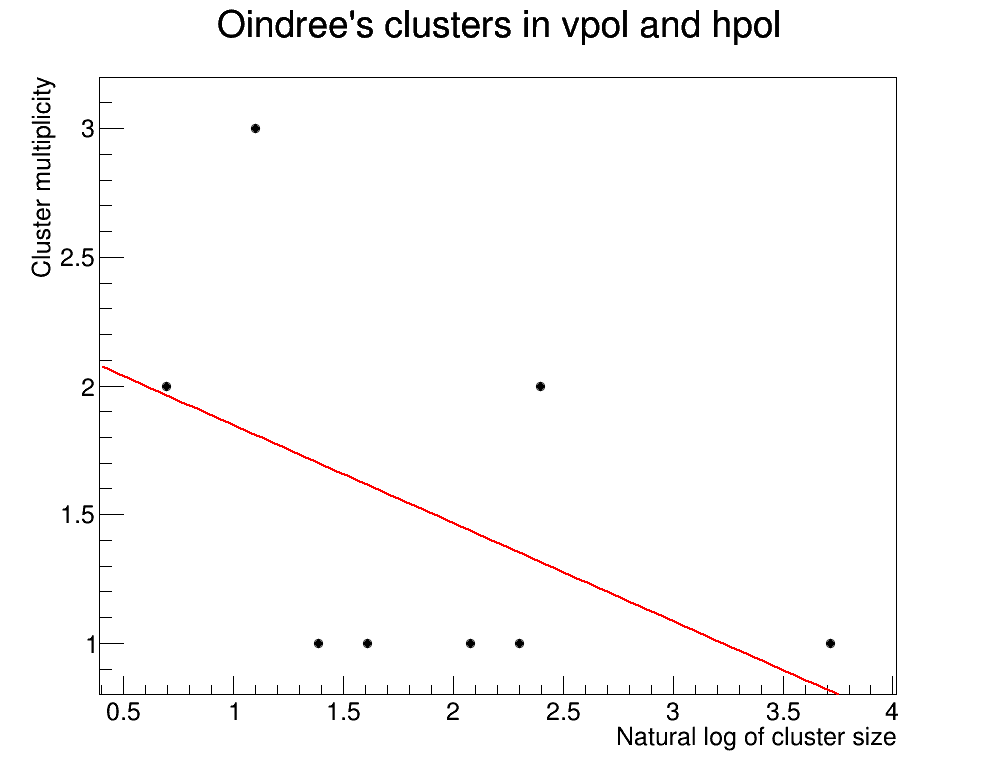
\includegraphics[width=1.0\textwidth]{figures/clusterSizeVsMultiplicity.png}
\caption{Cluster multiplicity as a function of cluster size. The fit to this distribution was used to calculate a background estimate from the clustering cut.}
\label{cluster_mul}
\end{figure}


\begin{figure}
\centering
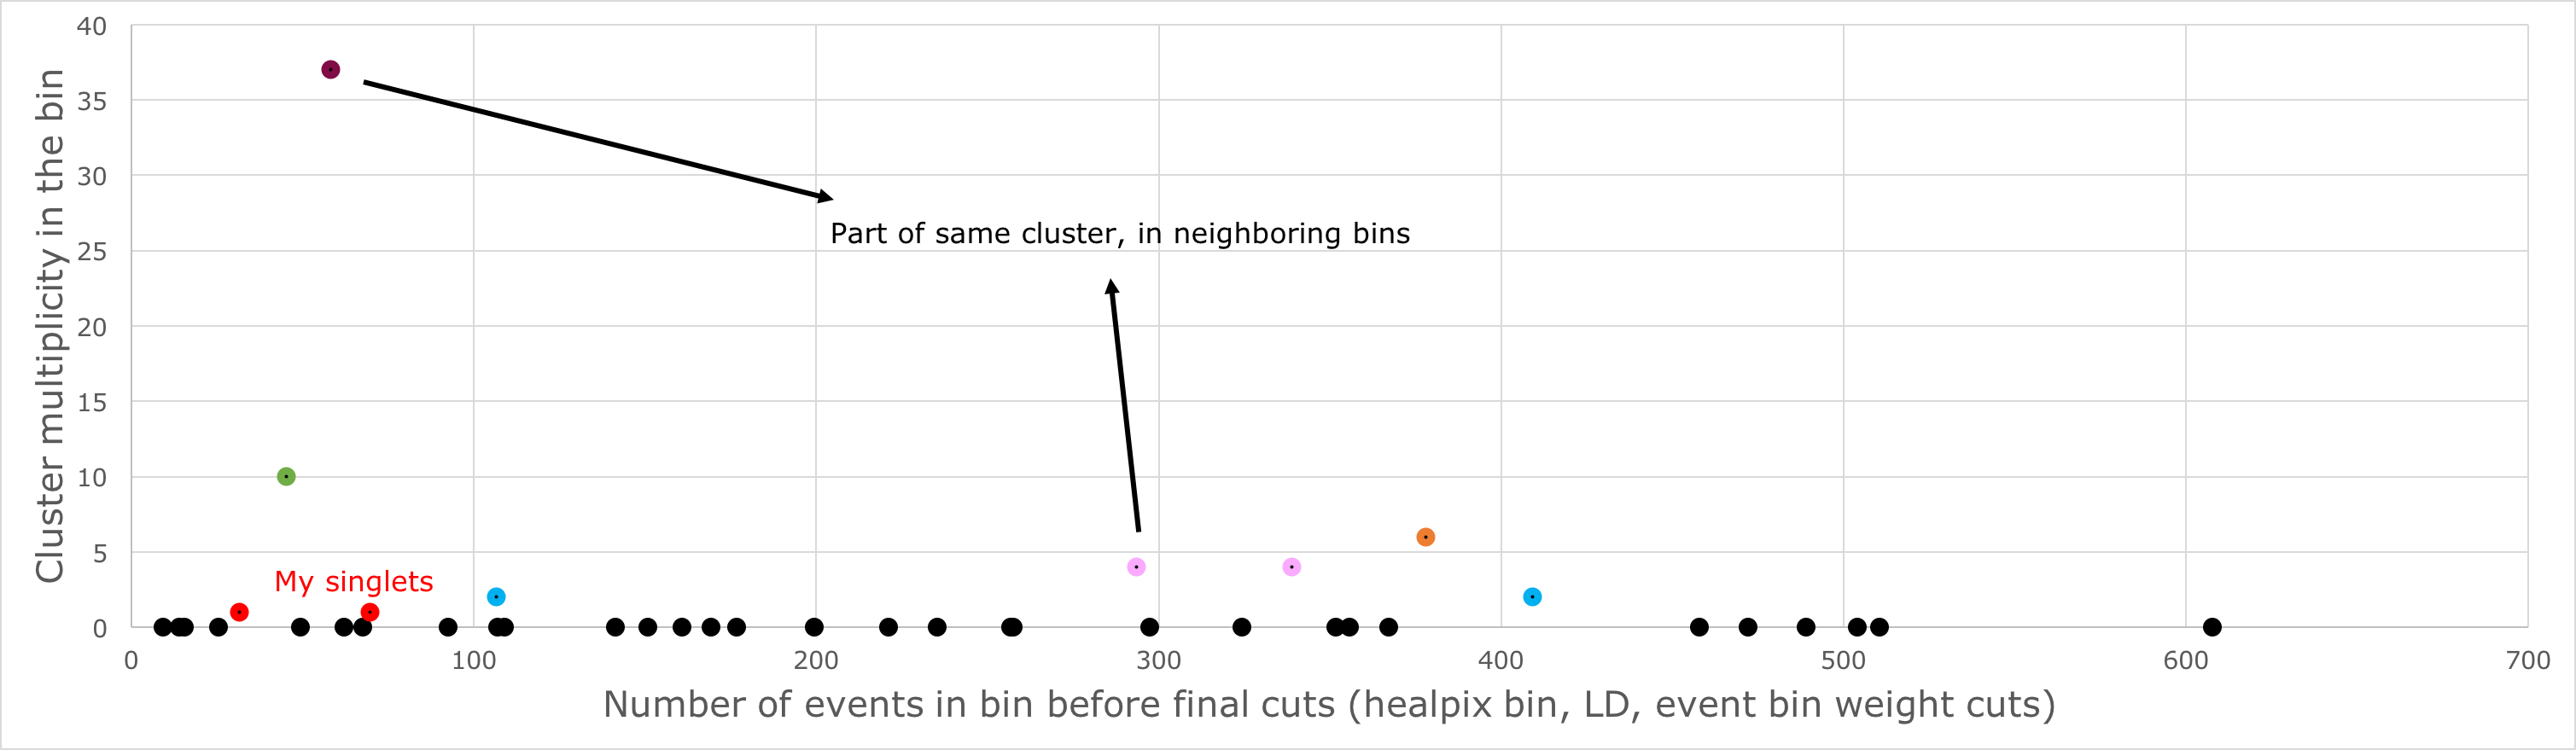
\includegraphics[width=1.0\textwidth]{figures/clusterMultiplicityVsEventPopulationBeforeFinalCuts.png}
\caption{Cluster size as a function of event population before final cuts in the VPol analysis. There does not appear to be a trend suggesting a greater likelihood of finding clusters in bins with more events before final cuts. This is an important validation of the binned analysis.}
\label{cluster_pop}
\end{figure}

\section{Complementary efficiency}

The efficiency of the analysis is calculated using the number of simulated neutrinos that pass all cuts. The efficiency of the binned analysis was 6.91\%, after accounting for efficiency loss due to clustering. Although this efficiency is low and needs to be improved in the future, a large fraction of this efficiency is complementary to that of one of the clustering analyses (Analysis A) described in~\cite{diffuse}. This was found by calculating the number of neutrinos that was kept in the binned analysis which was not kept in the complementary analysis. 

The number of neutrinos kept in the binned analysis that the complementary analysis did not keep was 35.9 (for a given number of neutrinos thrown in the Monte Carlo) and the total number of neutrinos kept in the binned analysis was 142.3. Therefore, 25.2\% of the neutrinos kept in the binned analysis was not kept in the complementary analysis. This 25.2\% of the efficiency of the binned analysis is, therefore, complementary and can be added to the other analysis. The efficiency that would be added is calculated to be 1.7\%, which is small but not insignificant. If the overall efficiency of the binned analysis were to improve, its complementary efficiency which could be directly added to the efficiency of other analyses would be greater as well. 


\section{Blastfamy: Team effort to remove payload blasts}
\label{blastfamy}

I developed a project called Blastfamy to guide undergraduate students through the process of learning how to use \gls{anita} analysis tools and to apply that towards finding payload blast specimens in the data. These blasts would then be used as a training sample to perform an analysis potentially involving machine learning to remove all such blasts from the dataset. An example of a blast event can be seen in Figure~\ref{blast}. 

\subsection{Principal Component Analysis}

I performed some tests with the \gls{anita}-3 data to determine the potential of blast removal with unsupervised methods such as \gls{pca}, following valuable communication on the topic with Brian Connolly. I used a spreadsheet having the values of 10 features of events from the \gls{anita}-3 data and performed a \gls{pca} on it with R. Results from this can be seen in Figures~\ref{pc} and~\ref{pca}. 

\gls{pca} is an analysis technique mainly used to reduce the dimensionality of a multi-dimension dataset. In my test, the initial dimension of the dataset is 10. The \gls{pca} successfully reduces this by calculating linear combinations from the features and determining which linear combinations can describe the data the best. The coefficients of the features in the linear combinations can be seen in Figure~\ref{pc}. Ten principal components are calculated here using linear combinations of the 10 features. It can be seen from the bottom plot that the first two or three principal components are the most important ones as the variances associated with each one fall off exponentially. This is how \gls{pca} is able to reduce the dimensionality of the problem. 

The first two principal components are plotted in the top plot of Figure~\ref{pca}. The resulting image resembles a knee. In this ``knee plot", we can see that there are a group of events in the bottom left, separated from the main knee. These bottom left events on the knee plot were checked. They were not blasts, and instead looked thermal-like to me. There is also a tail present in the knee plot and the events in this tail were also checked. The tail events were all low-quality events such as digitizer glitches. An example each of the bottom left events and tail events can be seen in Figure~\ref{bottom_tail}.
The knee plot was re-made with a few known blast events overlaid. These events were in the thick of the knee and not easily separable as seen in Figure~\ref{blasts_over}. From this, I concluded that more work needed to be done to reject blasts following these methods.

\subsubsection{Future}

This method of \gls{pca} can certainly be improved, for example, by using more and better features. A quick test with 27 features yielded the variances shown in Figure~\ref{var_new}. A more advanced method of analysis such as a Linear Discriminant Analysis, which is a semi-supervised method, could also be implemented in the future by using the principal components generated from features of a sample of all blast events as the training dataset. 

\begin{figure}
\centering
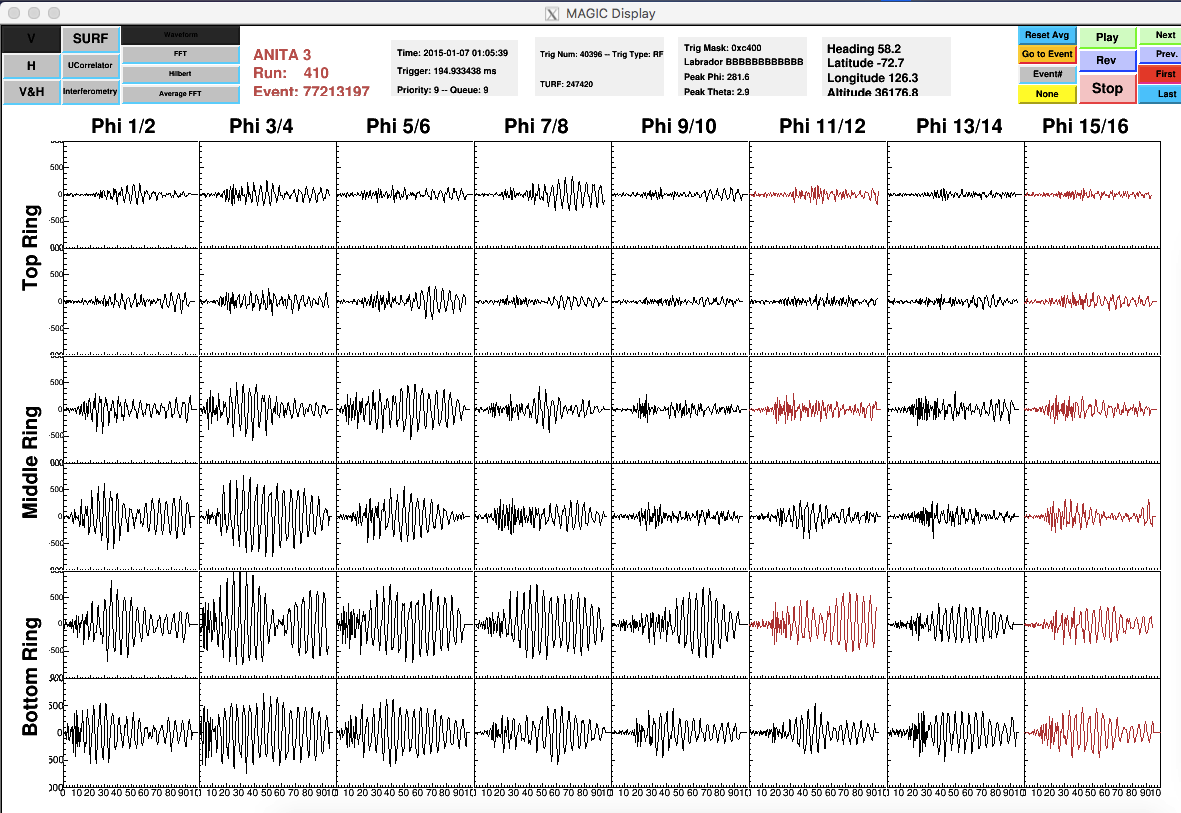
\includegraphics[width=1.0\textwidth]{figures/77213197.png}
\caption{Example of a payload blast event. Waveforms received by all antennas in VPol are shown here.}
\label{blast}
\end{figure}

\begin{figure}
\centering
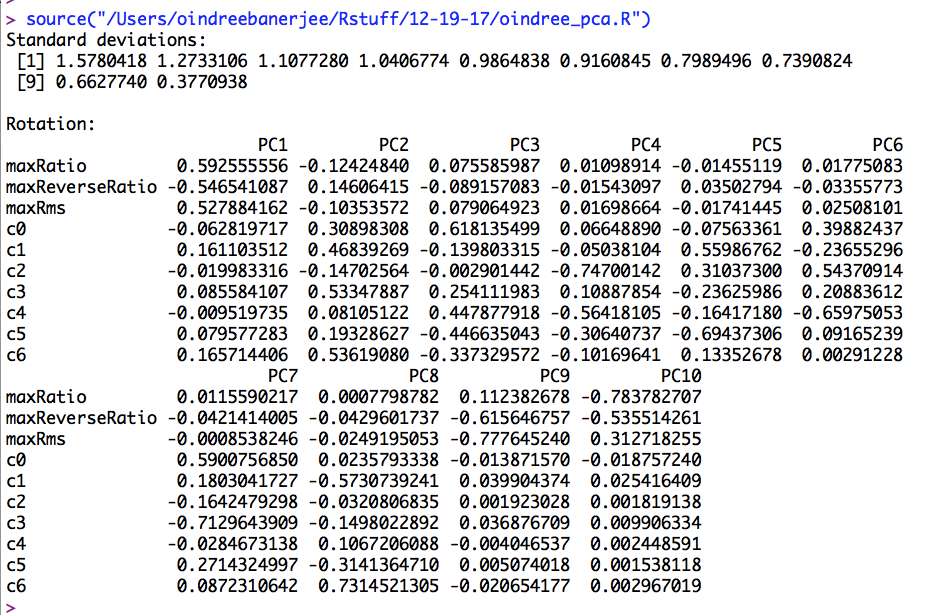
\includegraphics[width=1.0\textwidth]{figures/PCs.png}
\caption{PCs printed out.}
\label{pc}
\end{figure}

\begin{figure}
\centering
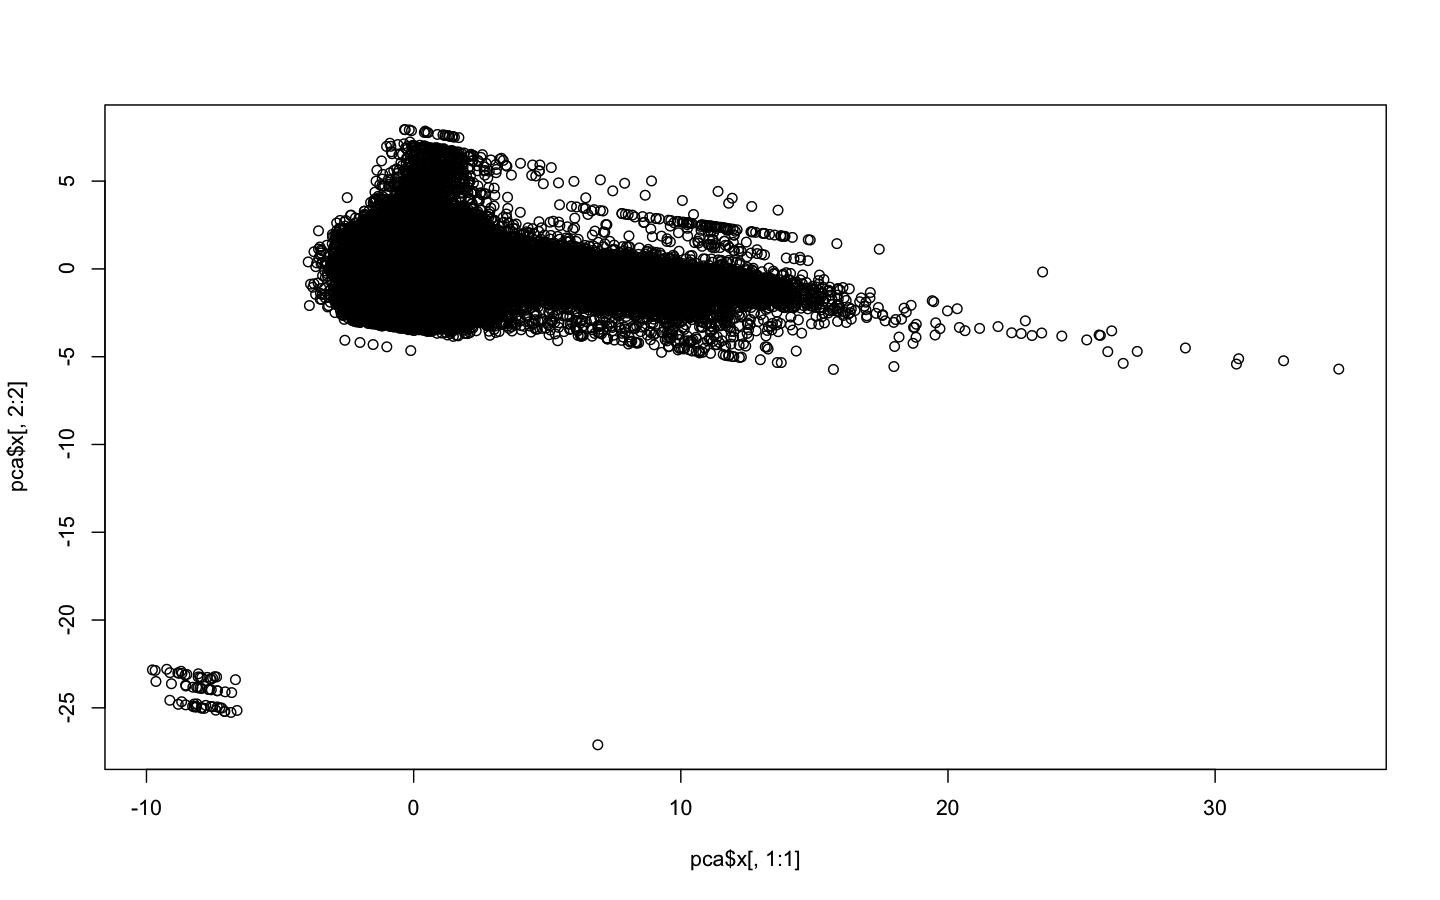
\includegraphics[width=1.0\textwidth]{figures/pca_plot.png}
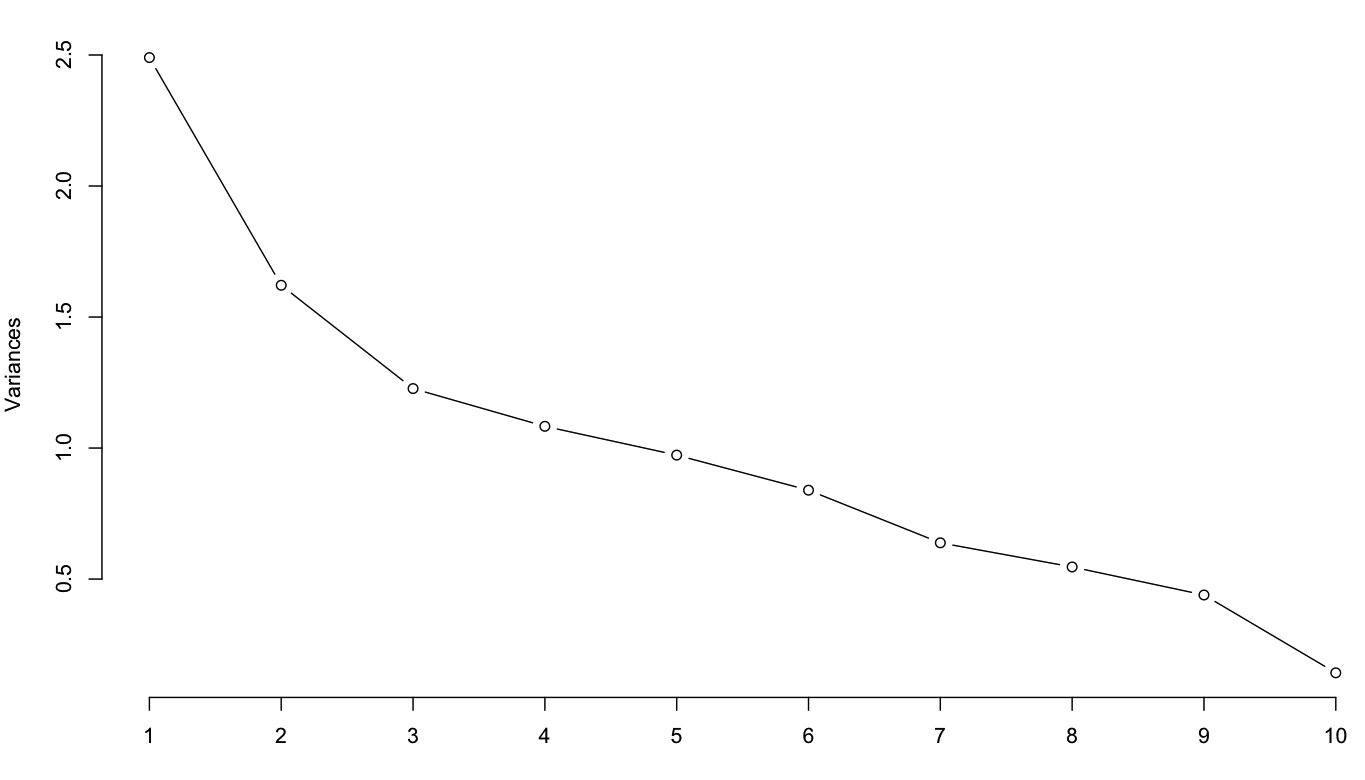
\includegraphics[width=1.0\textwidth]{figures/pca_variances.png}
\caption{Principal components and variances using 10 features. The knee plot is presented at the top here.}
\label{pca}
\end{figure}


\begin{figure}
\centering
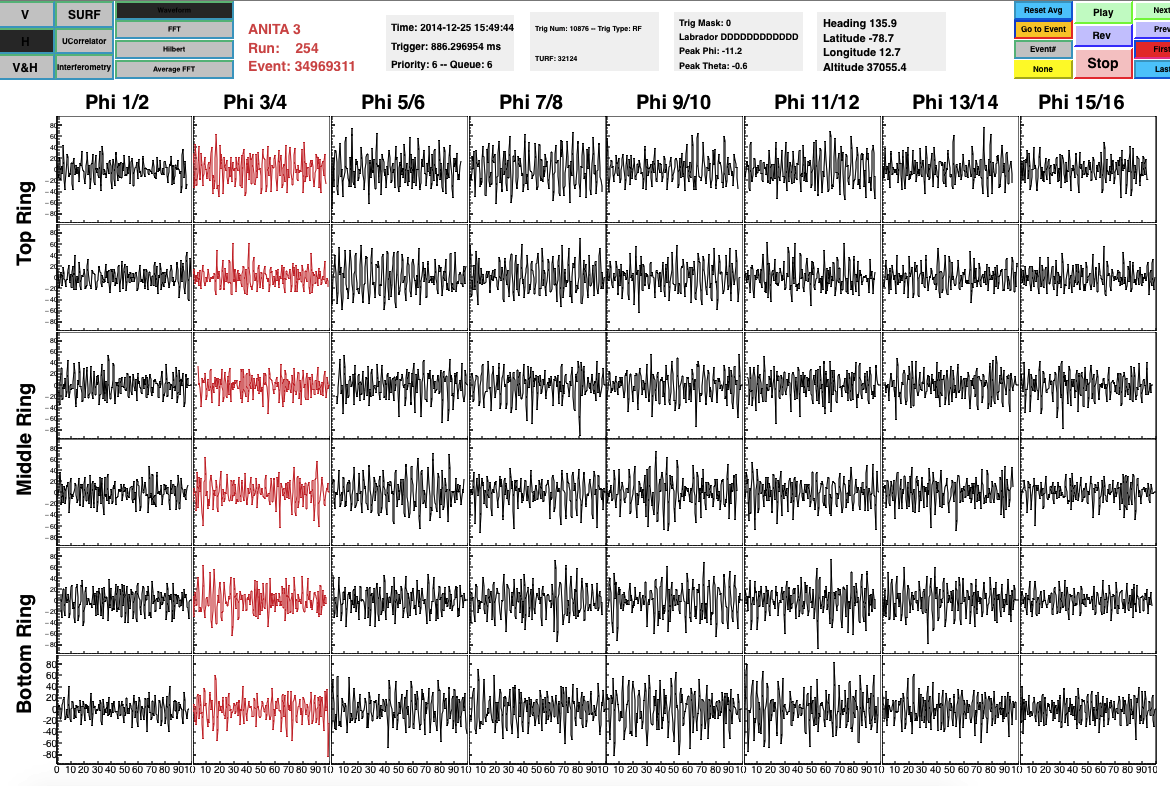
\includegraphics[width=0.9\textwidth]{figures/bottom_left_ex.png}
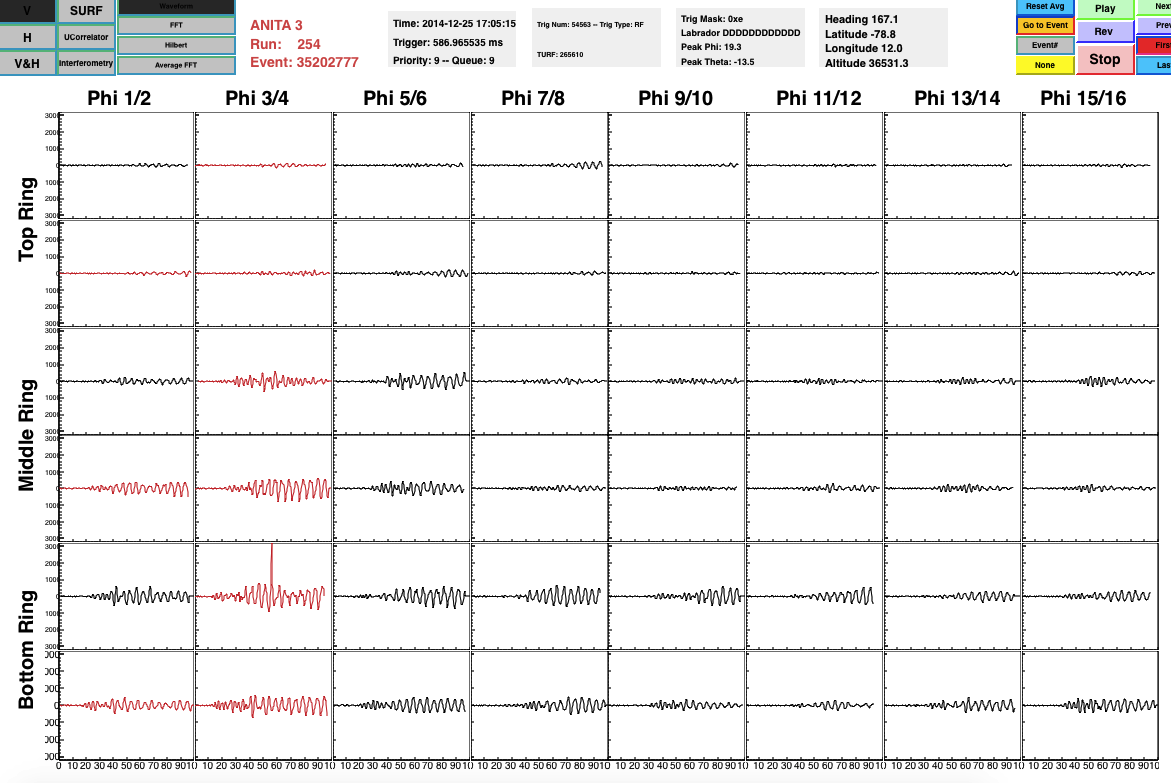
\includegraphics[width=0.9\textwidth]{figures/tail_event_ex.png}
\caption{Example of a bottom left event from the knee plot (top) and tail event from the knee plot (bottom).}
\label{bottom_tail}
\end{figure}


\begin{figure}
\centering
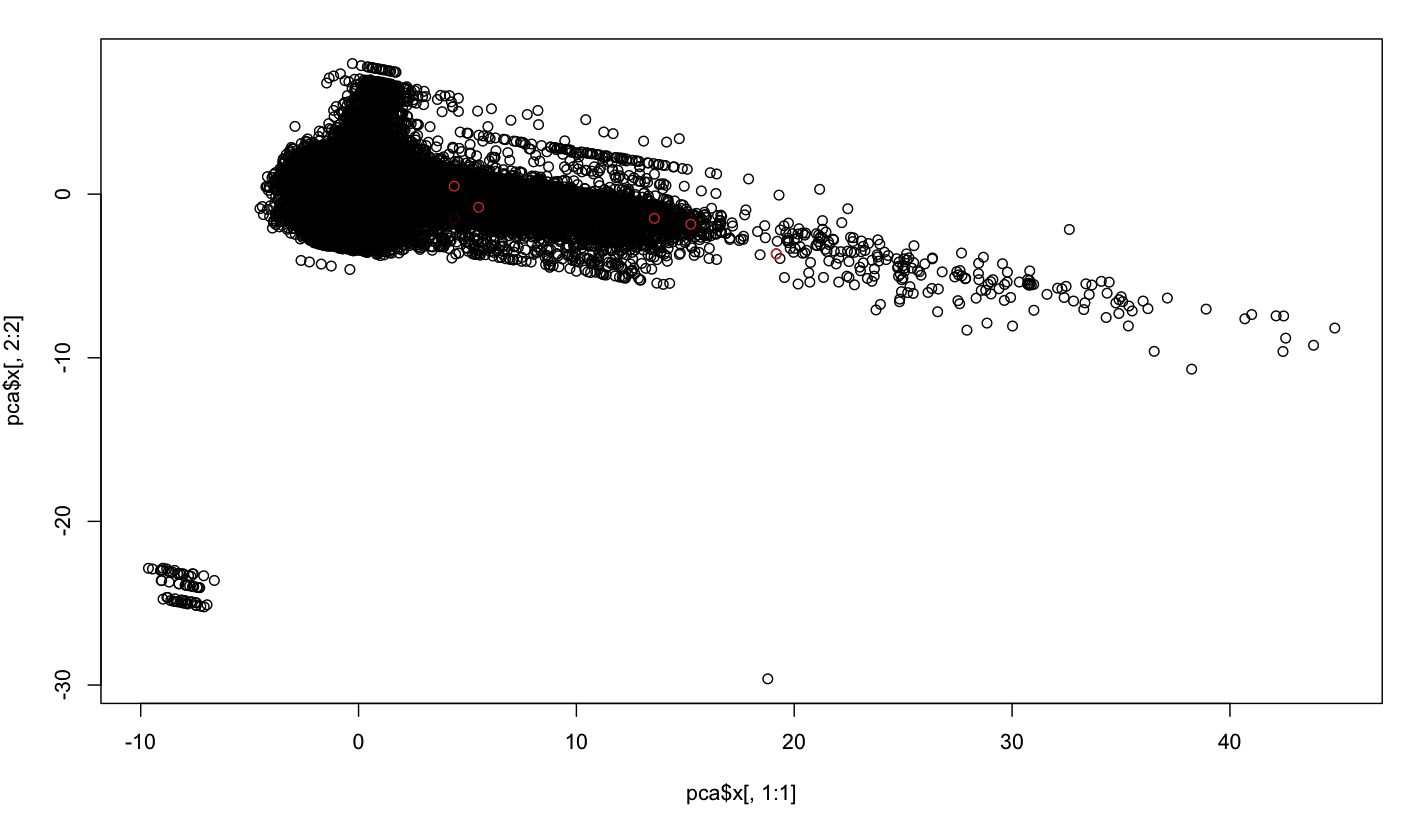
\includegraphics[width=1.0\textwidth]{figures/kneePlotWithBlastsOverlaid.png}
\caption{Blasts overlaid on knee plot. }
\label{blasts_over}
\end{figure}


\begin{figure}
\centering
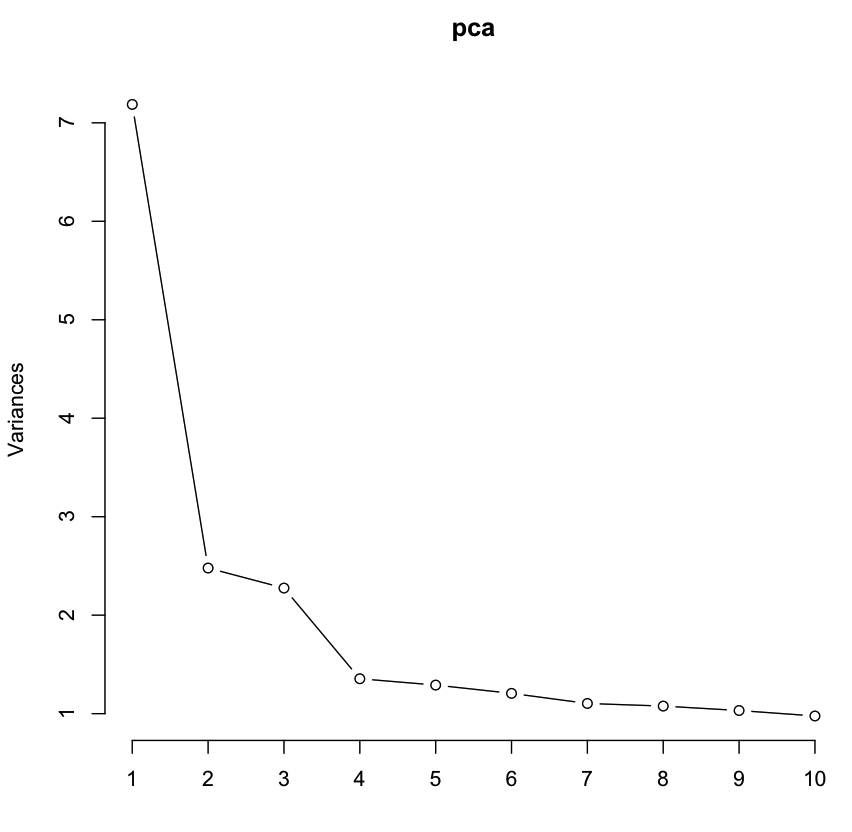
\includegraphics[width=1.0\textwidth]{figures/pca_variances_new.png}
\caption{Variances from using 27 features.}
\label{var_new}
\end{figure}












